\section{Results}
Following the procedure described in the Algorithm \ref{alg:alg1},
we can obtain the vector $\VECTOR{\hat{c}}$ that optimize the model fitting of 
$f_{\VECTOR{\hat{c}}}(\VECTOR{x})$ between the training information;
so that
\begin{equation}
\VECTOR{\hat{c}}=
\begin{bmatrix}
0.13510 & -0.24261 &  0.10244 & -1.95836
\end{bmatrix},
\end{equation}
and consequently
\begin{equation}
f_{\VECTOR{\hat{c}}}(\VECTOR{x})=\frac{1}{1+e^{-0.13510 + 0.24261 x_1 -0.10244 x_2 + 1.95836 x_3}}.
\end{equation}

A Fig. \ref{fig:planecoef} shows two sets, of $N$ points each one, 
selected randomly in the Fig. \ref{fig:data-trainning-bw},
the points $\VECTOR{x}$ drawn with the color red represent pixels in a coffee seeds, and
the points $\VECTOR{x}$ drawn with the color blue represent pixels that don't belong to a coffee seed.

\begin{figure}[h!]
\centering
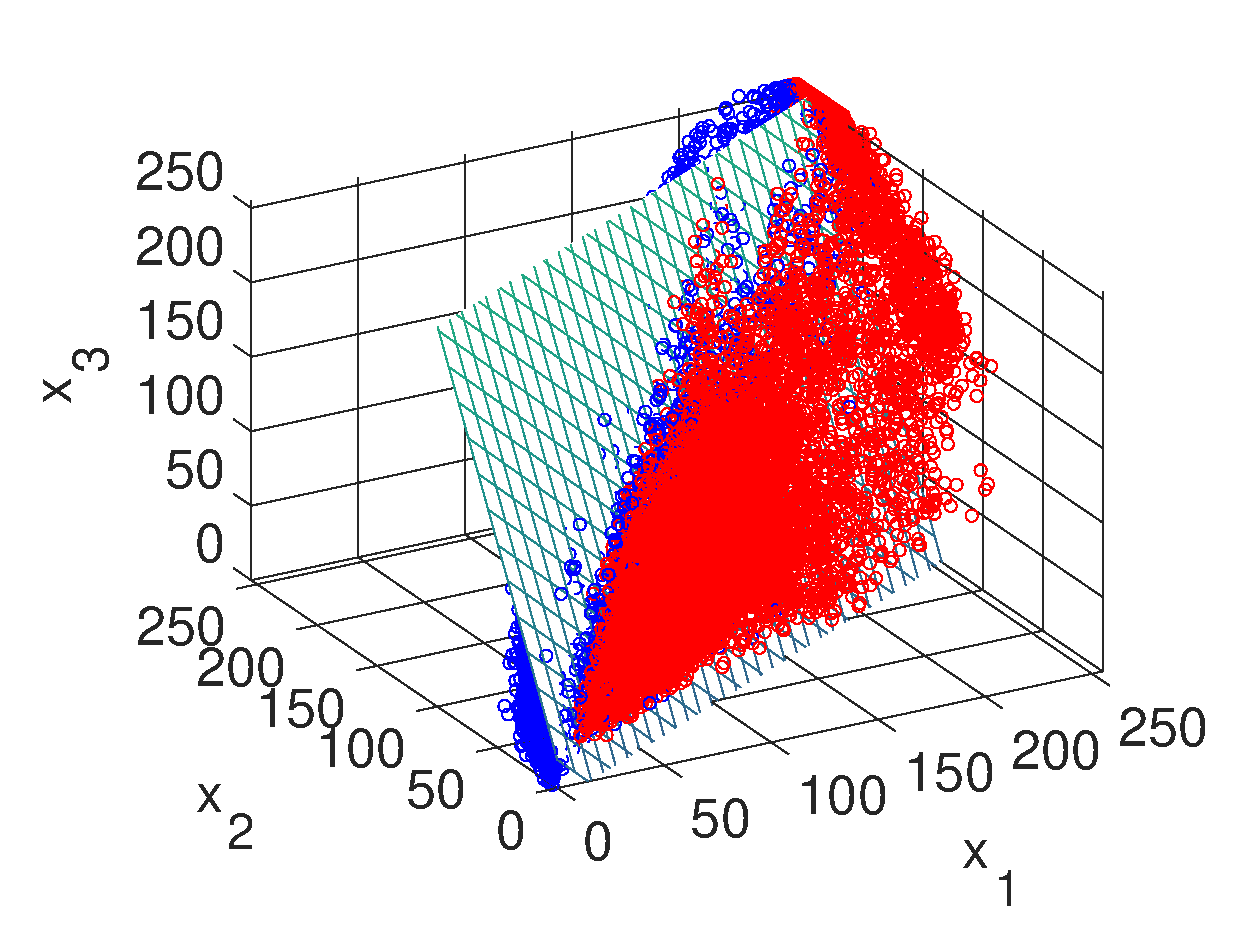
\includegraphics[width=0.99\linewidth]{plane_coef.eps}
\caption{Points $\VECTOR{x} \in \mathbb{R}^{3}$ and the hyperplane $h_{\VECTOR{\hat{c}}}(\VECTOR{x})=0$.}
\label{fig:planecoef}
\end{figure} 

The Fig. \ref{fig:sigmoid_result} shows the result of evaluate each pixel $\VECTOR{x}$ of Fig. \ref{fig:data-color}
with the function $f_{\VECTOR{\hat{c}}}(\VECTOR{x})$.
Thus, the resulting image have values between $0$ and $1$,
and was colorized with a color map with colors between blue and red 
to show results $0<y<1$.
\begin{figure}[h!]
\centering
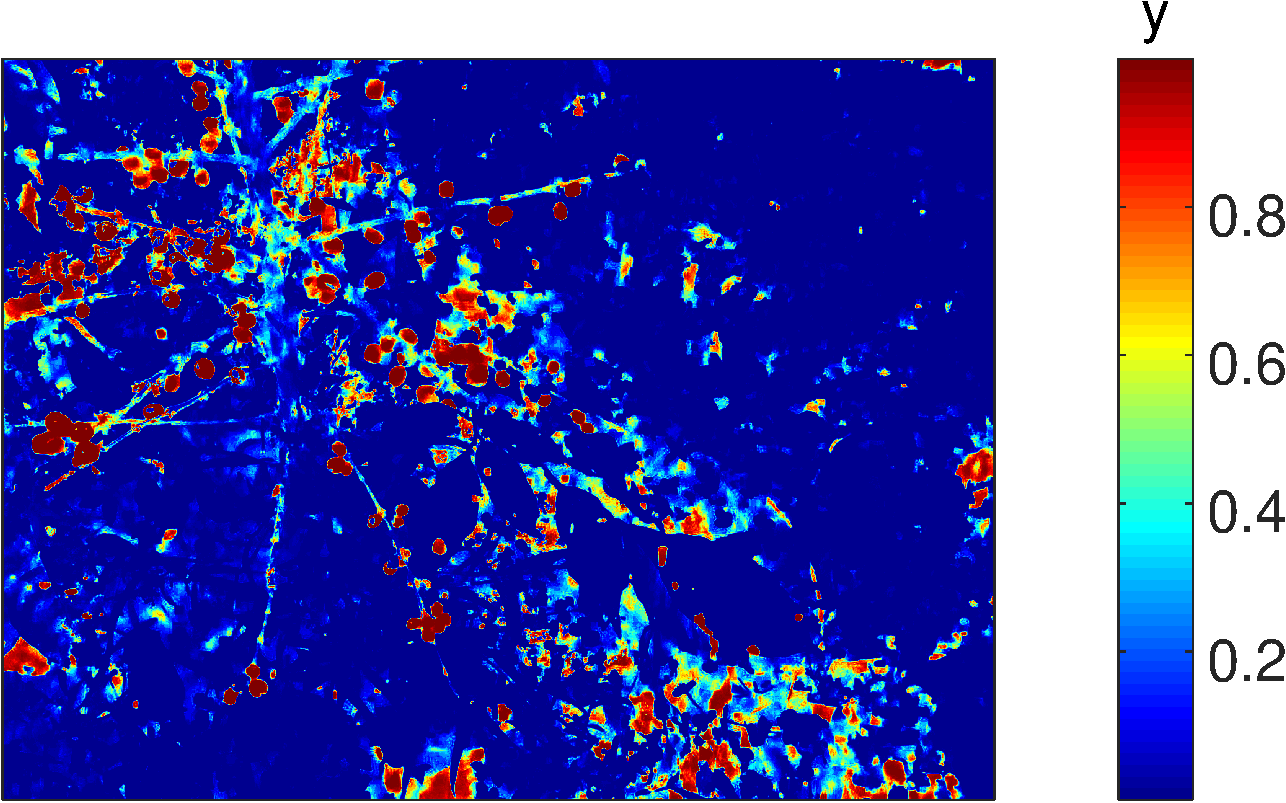
\includegraphics[width=0.99\linewidth]{sigmoid_result.png}
\caption{Result of function $f_{\VECTOR{\hat{c}}}(\VECTOR{x})$.}
\label{fig:sigmoid_result}
\end{figure} 
